Наступні результати були отримані за допомогою мови програмування Python
її бібліотек PyTorch та PyMaxflow. Наступні тестування проводились на комп'ютері з
процесором Intel Core i5-7200U @ 4x 3,1GHz на операційній системі Ubuntu 21.04.


\section{Результати алгоритму Б-К та згорткових мереж}

В даній роботі досить непогано проявив себе метод Б-К, а саме програмна бібліотека
PyMaxflow автором якої є сам Колмогоров. Даний метод найшвидше працює саме в ній.


\begin{figure}[H]
    \centering

    \subfloat[]{
        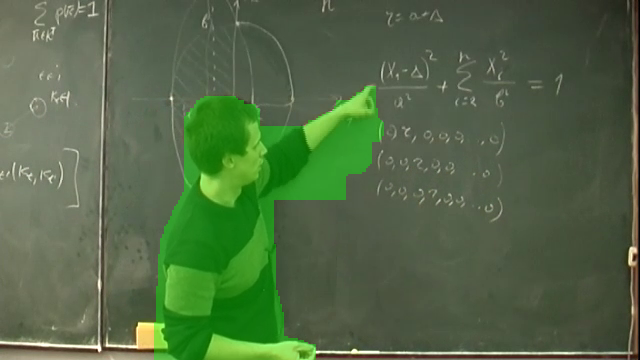
\includegraphics[width=0.35\textwidth]{images/convex_11_bk_10600}
    }
    \subfloat[]{
        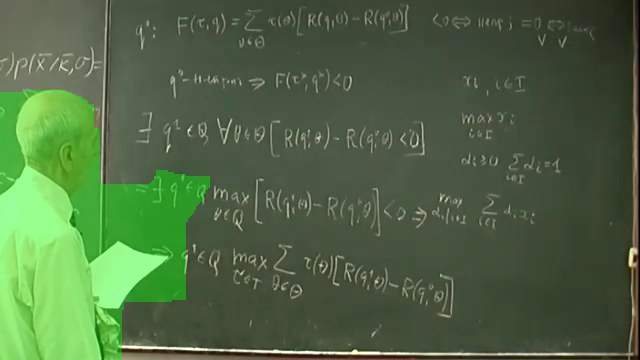
\includegraphics[width=0.35\textwidth]{images/schlezinger_bk_6500}
    }\\
    \subfloat[]{
        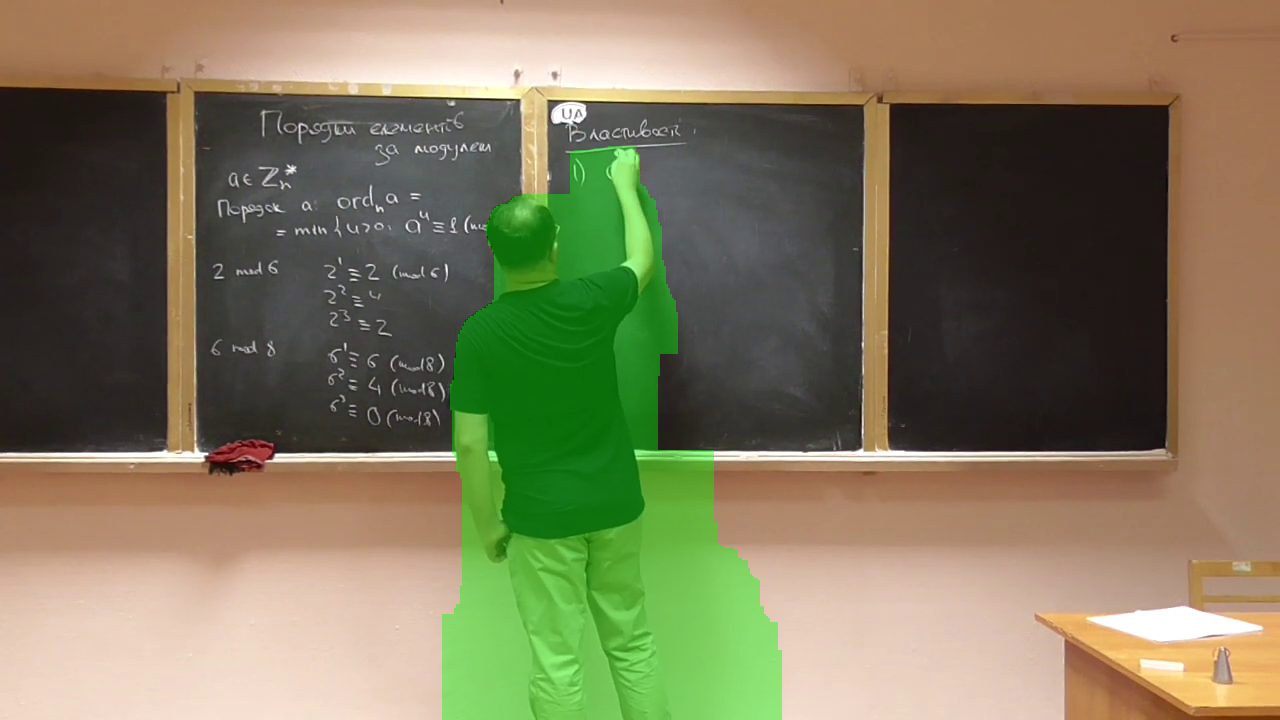
\includegraphics[width=0.35\textwidth]{images/yakovlev2_bk_6500}
    }
    \subfloat[]{
        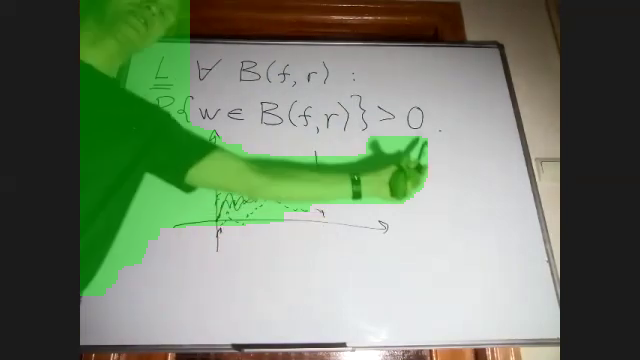
\includegraphics[width=0.35\textwidth]{images/dorohovtsev2_bk_10650}
    }
    \caption{Приклад роботи алгоритму Б-К для отримання маки рухомих об'єктів
        \label{fig:bk_examples}
    }
\end{figure}


Як ми бачимо на прикладах (Рис. \ref{fig:bk_examples}) досить гарна якість маски рухомих об'єктів.

\textbf{Переваги методу:}
\begin{enumerate}
    \item Алгоритм Б-К досить швидко будує мінімальний розріз. Статистика на ОС
          під, час 0.15 секунди на кадр розміром 330х640.
    \item Даний метод не потребує ніякої передобробки, тобто не потрібно навчати
          як нейронну мережу.
\end{enumerate}

\textbf{Недоліки методу:}
\begin{enumerate}
    \item Оскільки даний метод локалізує рух на кадрах відео, то коли
          рухається камера, відповідно практично все що в кадрі стає рухомим об'єктом
          (Рис.\ref{fig:bk_bad_mask}).
          Частково дана проблема вирішена на 2-му кроці алгоритму створення панорами
          (Алгоритм \ref{al:panorama_creating_algorithm}).
          \begin{figure}[H]
              \centering

              \subfloat[]{
                  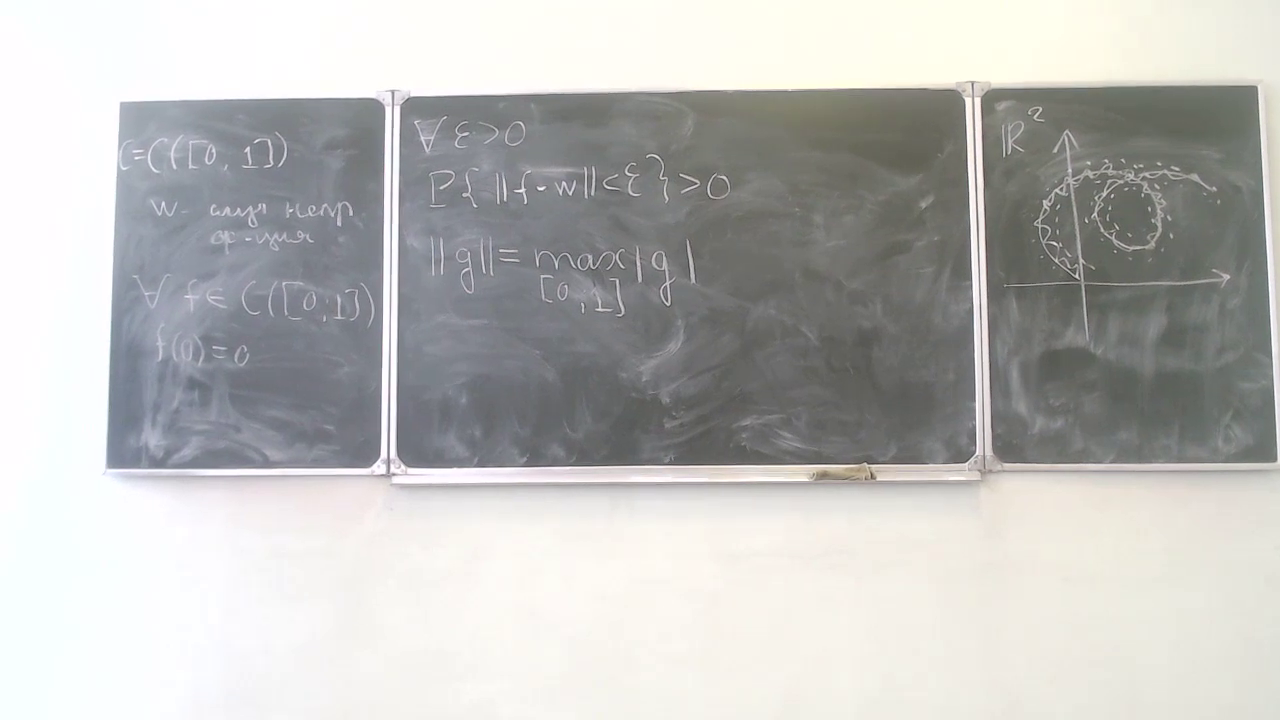
\includegraphics[width=0.35\textwidth]{images/bad_prev_dorohovtsev_bk_5790}
              }
              \subfloat[]{
                  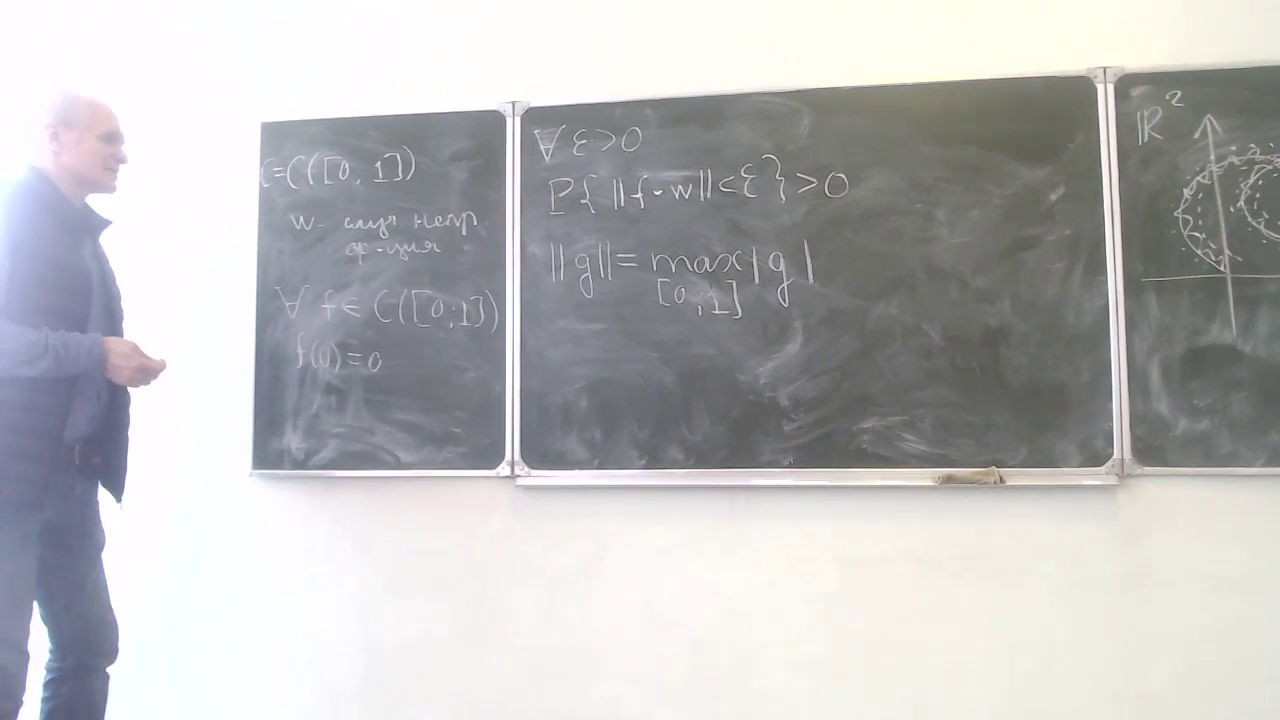
\includegraphics[width=0.35\textwidth]{images/bad_next_dorohovtsev_bk_5840}
              } \\
              \subfloat[]{
                  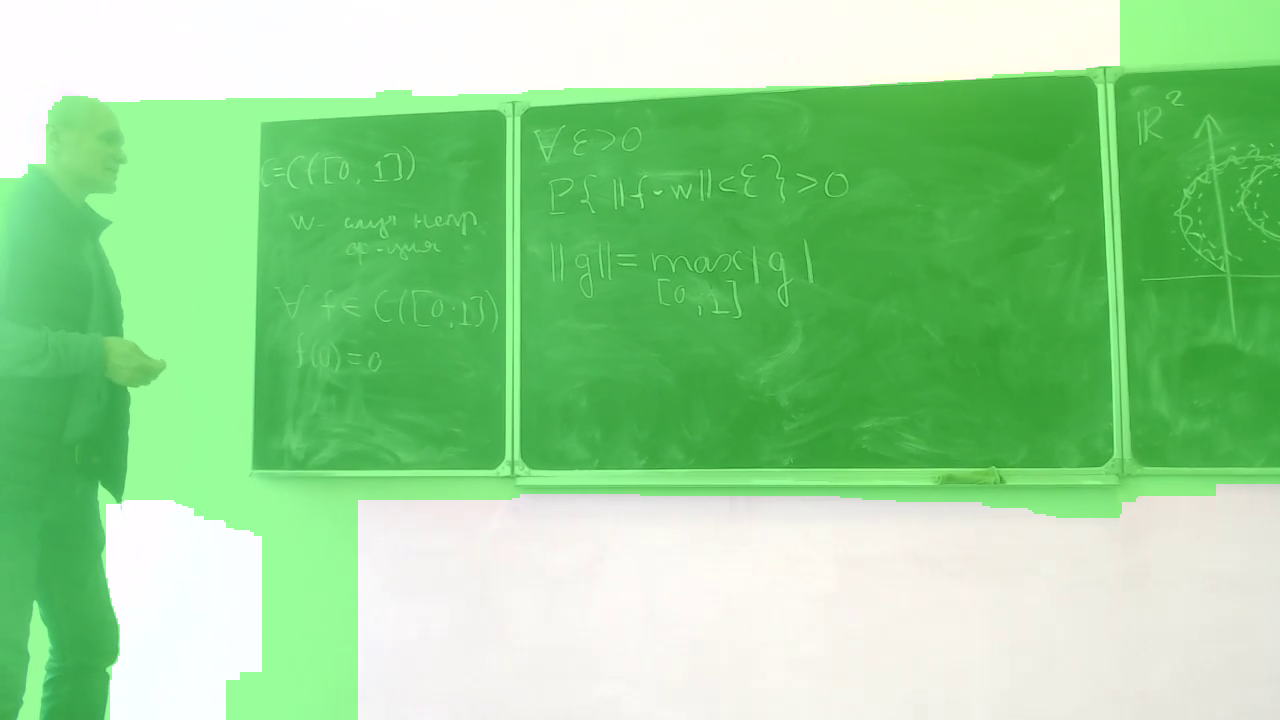
\includegraphics[width=0.35\textwidth]{images/bad_dorohovtsev_bk_example_5840}
              }
              \caption{Приклад поганої маски рухомих об'єктів
                  \label{fig:bk_bad_mask}
              }
          \end{figure}

    \item Якщо викладач практично не рухається довгий час, відповідно частково не потрапляє
          на маску рухомих об'єктів, з цього слідує, що він може потрапити на панорамний слайд.
\end{enumerate}


\section{Результати згорткових мереж}

\begin{figure}[H]
    \centering
    % yolov5n
    \subfloat[]{
        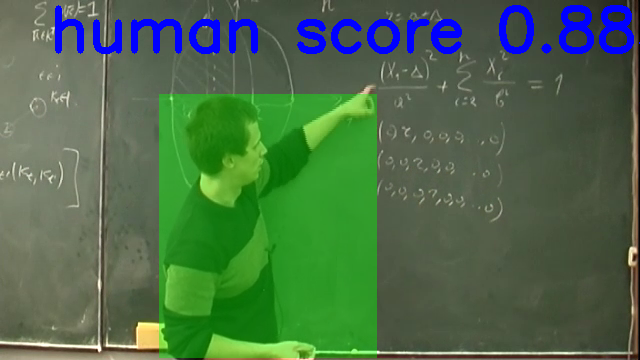
\includegraphics[width=0.35\textwidth]{images/convex_11_yolov5n_10600}
    }
    \subfloat[]{
        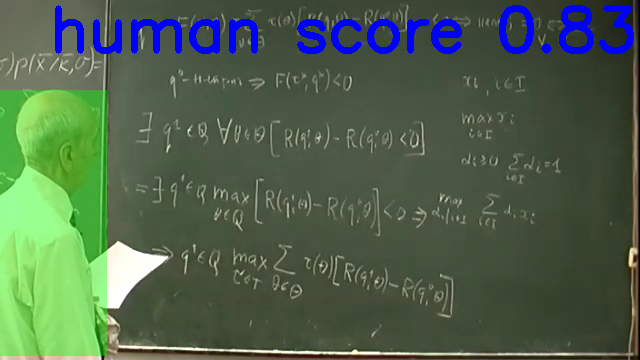
\includegraphics[width=0.35\textwidth]{images/schlezinger_yolov5n_6500}
    } \\
    \subfloat[]{
        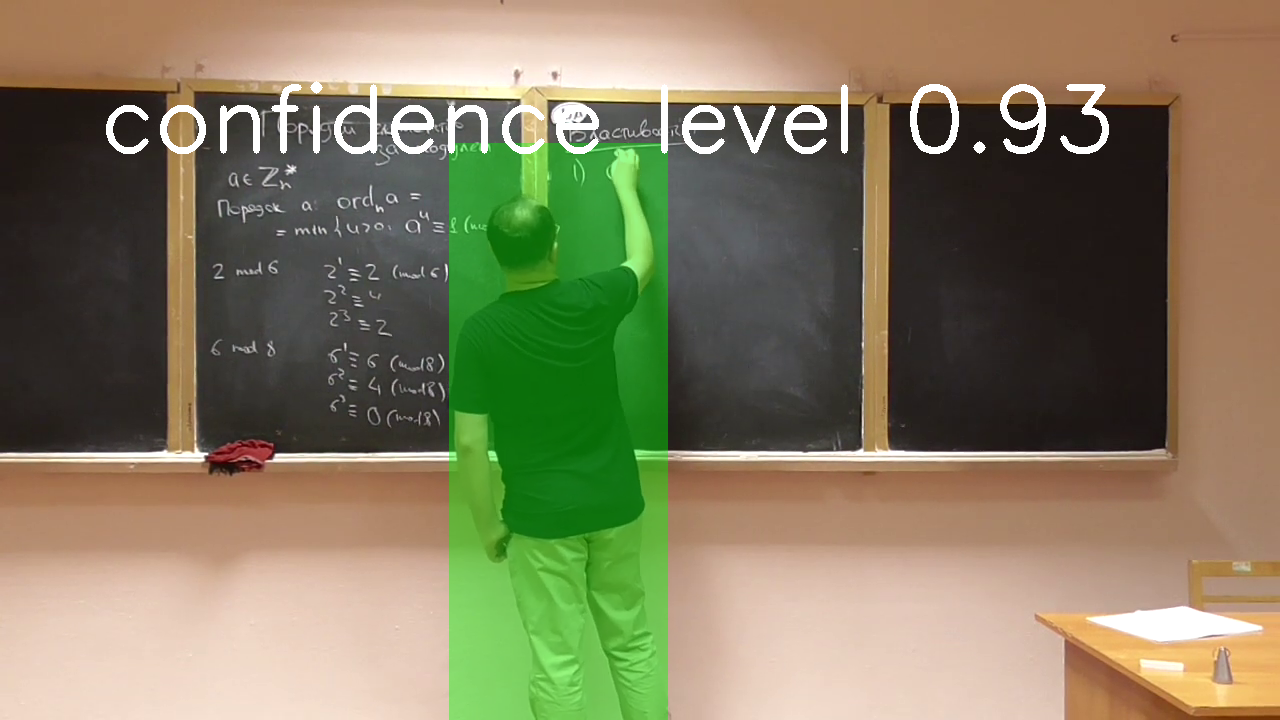
\includegraphics[width=0.35\textwidth]{images/yakovlev2_yolov5n_6500}
    }
    \subfloat[]{
        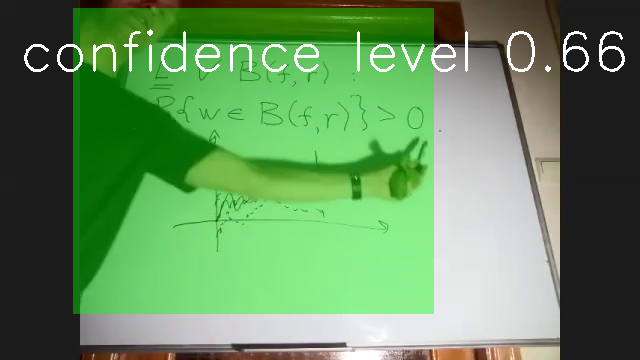
\includegraphics[width=0.35\textwidth]{images/dorohovtsev2_yolov5n_10650}
    }
    \caption{Приклад роботи yolov5n
        \label{fig:yolov5n_examples}
    }
\end{figure}

\begin{figure}[H]
    \centering
    \subfloat[]{
        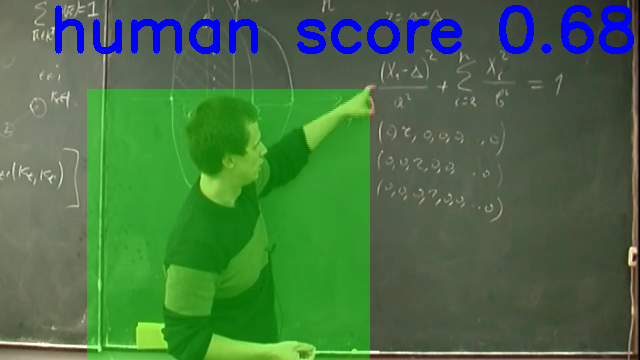
\includegraphics[width=0.35\textwidth]{images/convex_11_ssdlite320_mobilenet_v3_10600}
    }
    \subfloat[]{
        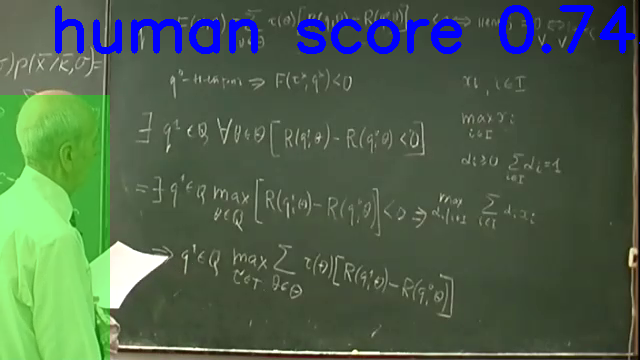
\includegraphics[width=0.35\textwidth]{images/schlezinger_ssdlite320_mobilenet_v3_6500}
    } \\
    \subfloat[]{
        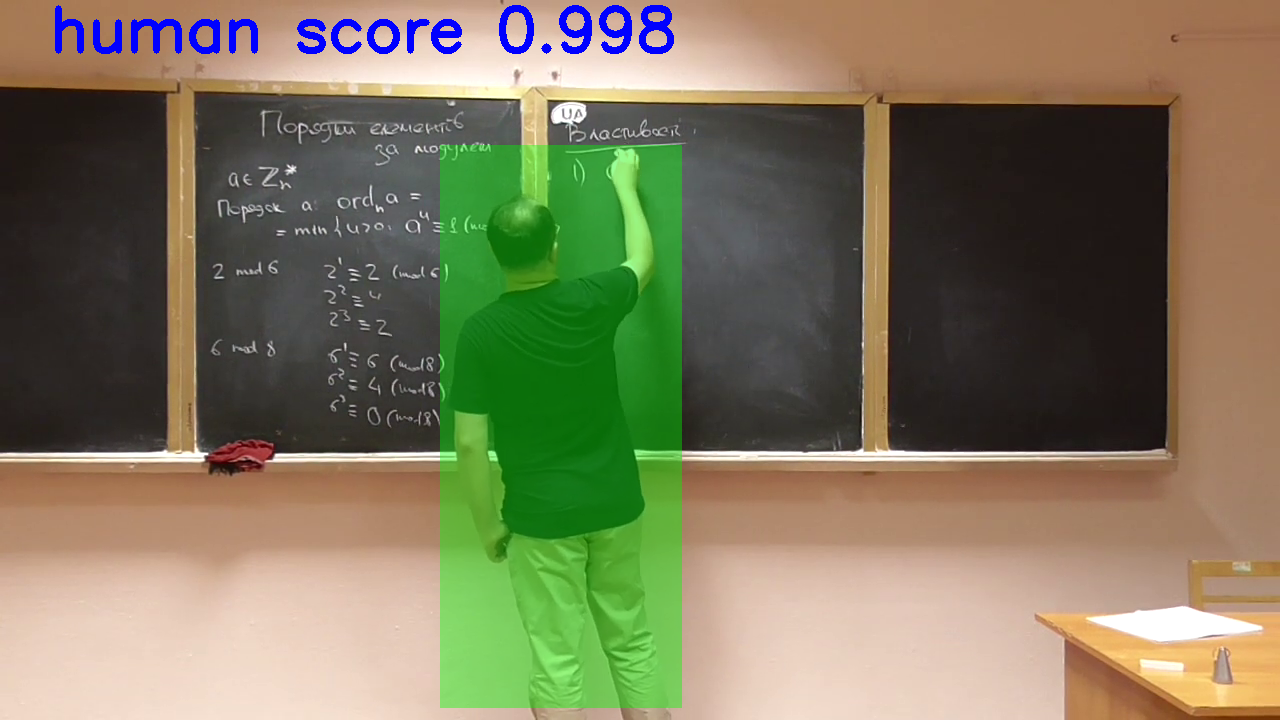
\includegraphics[width=0.35\textwidth]{images/yakovlev2_ssdlite320_mobilenet_v3_6500}
    }
    \subfloat[]{
        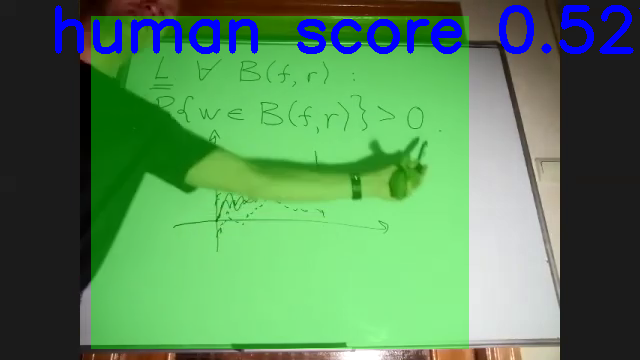
\includegraphics[width=0.35\textwidth]{images/dorohovtsev2_ssdlite320_mobilenet_v3_10650}
    }
    \caption{Приклад роботи ssdlite320-mobilenet-v3
        \label{fig:ssdlite320_mobilenet-v3_examples}
    }
\end{figure}

\begin{figure}[H]
    \centering
    \subfloat[]{
        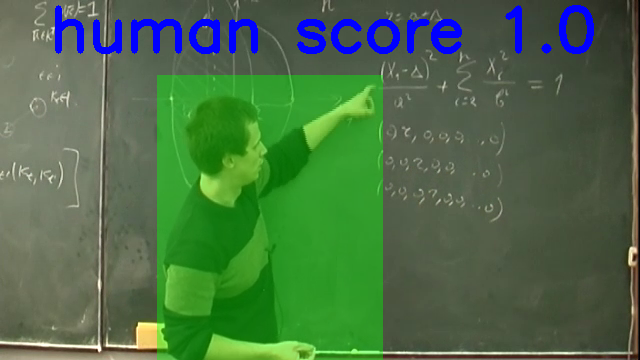
\includegraphics[width=0.35\textwidth]{images/convex_11_fasterrcnn_mobilenet_v3_10600}
    }
    \subfloat[]{
        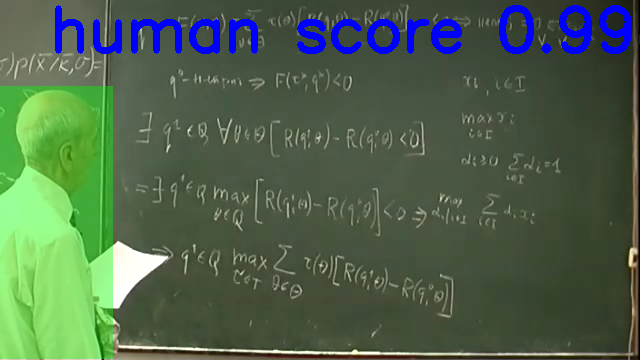
\includegraphics[width=0.35\textwidth]{images/schlezinger_fasterrcnn_mobilenet_v3_6500}
    }\\
    \subfloat[]{
        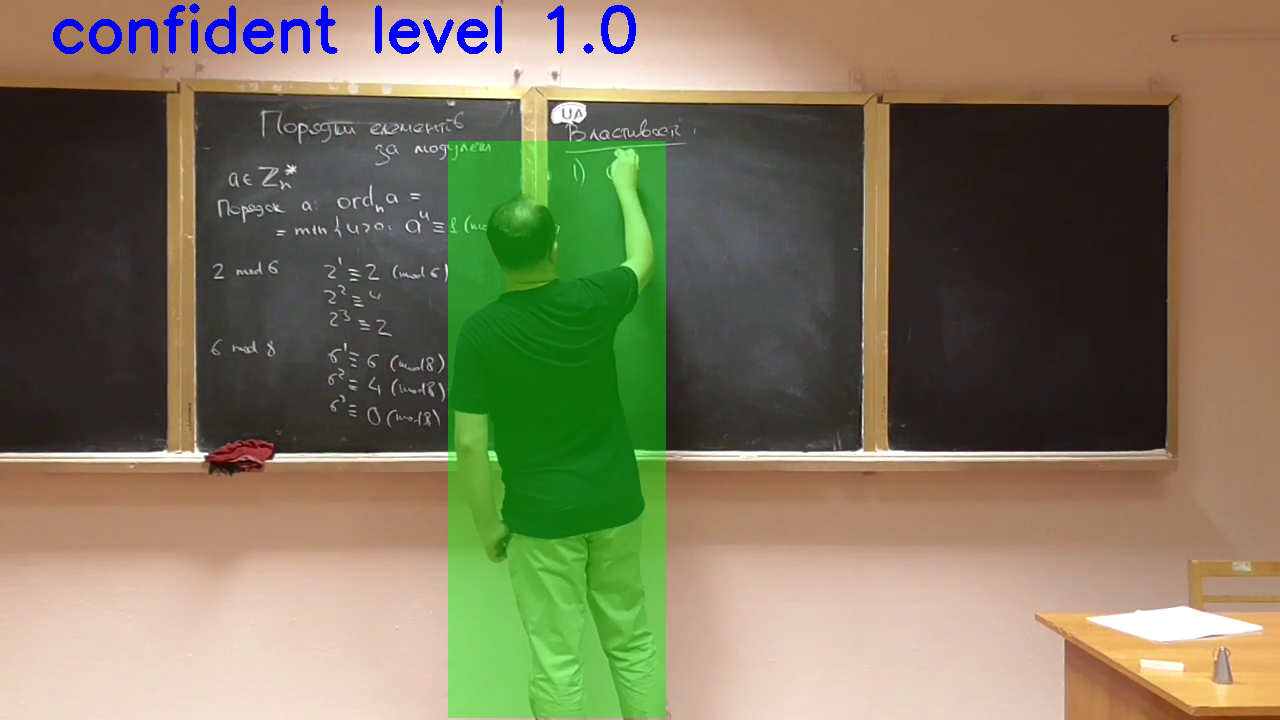
\includegraphics[width=0.35\textwidth]{images/yakovlev2_fasterrcnn_mobilenet_v3_6500}
    }
    \subfloat[]{
        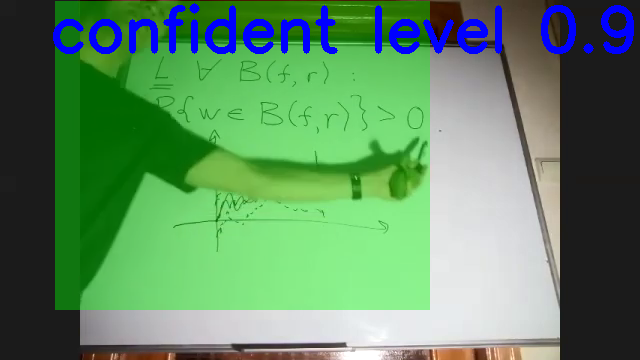
\includegraphics[width=0.35\textwidth]{images/dorohovtsev2_fasterrcnn_mobilenet_v3_10650}
    }
    \caption{Приклад роботи fasterrcnn-mobilenet-v3
        \label{fig:fasterrcnn_examples}
    }
\end{figure}


\textbf{Переваги згорткових мереж:}
\begin{enumerate}
    \item Згорткові мережі детекції людини, що були використані в даній роботі
          є теж досить швидкими, оскільки були створені для мобільних пристроїв.
    \item Детекція людини не залежить від руху камери. Відповідно навіть кадри, що
          отримуються під час руху камери будуть застосовані для створення панорами.
    \item Результати свідчать про високу точність локалізації викладача.
\end{enumerate}

\textbf{Недоліки згорткових мереж:}
\begin{enumerate}
    \item Якщо викладач має в руці якийсь предмет, листок паперу чи маркер, то дані
          об'єкти мережа не локалізує, відповідно можуть бути дефекти на панорамі.
    \item Розмір інформаційної технології стає більшим через зберігання ваг.
\end{enumerate}


\section{Швидкість методів локалізації людини чи рухомих об'єктів}

Було протестовано 1000 разів отримання маски різними методами на картинці $720 \times 1280$ та 
отриманий середній час обробки кадру (Таб. \ref{tab:speed_methods_table}).
Варто відмітити, що картинка перед входом в шари згорток у згорткових мережах підлягають 
компресії до якогось базового розміру для входу. Така ж компресія робиться і для входу 
в алгоритм Б-К, картинка зменшується у двічі.

\begin{table}[H]
    \begin{center}
        \caption{Таблиця швидкості згорткових мереж та алгоритму Б-К}
        \label{tab:speed_methods_table}
        \begin{tabular}{l|c|c|r}
            \textbf{yolov5n} & \textbf{ssdlite320-mobilenet-v3} & \textbf{fasterrcnn-mobilenet-v3} & \textbf{Boykov-Kolmogorov} \\
            \hline
            0.125074         & 0.060158                         & 0.126397                         & 0.223045                             \\
        \end{tabular}
    \end{center}
\end{table}


Як бачимо найшвидшим методом є ssdlite320-mobilenet-v3, а найдовшим Бойкова-Колмогорова.
Але експерименти показали, що прийнятну якість дає саме yolov5n.

\section{Результати створення панорами}


